\section{Investigation Method}

As alluded to above the most useful metrics which currently exist to analyse parallel programs revolve around the program's span also know as it's \emph{Critical Duration}.

\subsection{Critical Duration Analysis}

The critical duration is the shortest possible time taken for a given parallel program to execute. This is often represented as \(T_\infty\) as it is equivalent to the execution time of a program if it were run on an infinite number of processors. The critical duration combined with the amount of total work a program does allows us to calculate the degree of parallelism which, as seen in Section \ref{section:cilkview}, will determine how scalable a program is. Scalability is a vital measurement in regards to parallel programming as the primary goal of parallel programming is to allow performance to increase as the number of processors available increase. 

\subsection{Measurement of Time}

When considering how this research would measure time two options were considered. The first is instruction count which is the method that Cilkview \cite{id8} adopts. They argue that because the advantages of adding another processor would only be realised if there was a large difference between parallelism and actual speed-up there is no need for a precise measurement of time. 

The other option was to attempt to take the actuate `wall clock' time measurements. The benefits of this include the fact that time is easily relatable to, meaning a programmer can quickly evaluate the output of the program and understand it. It can also be easily validated by external counters unlike instruction count. It was because of these reasons that this research decided to adopt this definition of time. 

Time was captured at a millisecond level to give an accurate result. This was chosen over cycles in order to increase portability and to ensure that changes brought about by CPU power saving options, such as CPU frequency being reduced, wouldn't affect the measurements. The method 'gettimeofday()' from the sys/time.h library was used over RDTSC \cite{id22} due to potential issues regarding CPU timers not being synchronised over multiple cores. 

A negative of this method of timing is the fact that it is it will take into account the entire host environment rather than the individual process. So, if the user is running the program on a machine which is heavily loaded, meaning it has a lot of running processes, the time measurements could be slower than on the same machine when it is dedicated to the program being analysed. This could affect the level of parallelism to be expected.

\subsection{Non-object Dependent Critical Duration Analysis}

The critical path algorithm devised in this research can be broken into two parts. Firstly the work first aspect, whereby object dependencies are ignored and, secondly, the object aware aspect. We will now discuss the details of both these aspects in turn.\\

\emph{Task Begins Execution}\\
The algorithm for obtaining the critical duration at run time without object dependencies can be seen in Figure \ref{fig:code_nodeps}. At first we calculate the parent's duration, this is done by subtracting the current time from the last set `start time' of the parent. This will either be the time at which parent was first executed or the time it was last resumed from a returning task. We then add the duration to the accumulation of work done by the parent to get the parent's current work done total. The parent's critical path is then updated. All work that parent has done on the current strand, that it's duration, will get directly added into it's critical path. The spawned/called task is assigned the parent's current critical duration instead of set to 0 as with the work done. We will see the reason behind this when object dependencies are introduced in Section \ref{section:obj_deps}.\\

\emph{Task Finishes Execution}\\
When a task is finished and returns to it's parent it's duration, work done and critical duration are calculated. The calculation of the critical duration takes into account the child's critical duration also. If a task has spawned children who have had a longer critical duration that the task its self then their critical duration should become it's critical duration. Once this has been determined the task's duration should be added to the critical duration because, like the parent tasks, the duration of a given task will always be a part of it's critical duration. 

The parent's critical duration is then calculated. This is determined by first deciding if the task that was executed can possibly be executed in parallel, that is, if it was called using a `spawn' method. If it can't then then the amount of work done will be added directly to its parent's critical duration. 

If the task can be run in parallel then its critical duration will be compared to the current highest child's critical duration for that parent. The child's critical duration is necessary because when the parent reaches a sync or ends, it's critical duration will be determined by comparing it's current critical duration and the highest critical duration of each of its children, allowing analysis tool to correctly represent spawn and sync statements. This will give us the final critical duration of any task.

Finally, when a task is finished execution its parent's total work is calculated. As this value is accumulation of all work done in a given strand and its children, the work done is simply added to the parent's current value for work done.\\

\emph{Sync Statement Called}\\
When a sync statement is called execution is stalled until all of the spawned tasks have returned. At this point, because we will record critical duration in serial execution, we know that all spawned tasks will have finished execution. We now want to re-evaluate the task's critical duration comparing it to the highest critical duration of it's children. The highest value will be the final critical duration of the task.

\begin{figure}
  \begin{lstlisting}[breaklines, showstringspaces=false]
  when each task is ready to execute:

     calculate parent's duration
     calculate parent's work done [p.wd + duration]
     calculate parent's critical path [p.cp + duration]     

     assign task's critical path = parent's critical path

  when a task is finished executing:

     calculate task's duration
     calculate task's work done [t.wd + duration]
     calculate task's critical duration: 
     	   t.cd = MAX(t.child_critical_duration, t.cd)
	   t.cd = t.cd + duration

     if the task hasn't been spawned:     
          calculate parent's critical duration:
	     p.cd = p.cd + duration
     else:
          calculate parent's child critical duration:
     	     p.ccd = MAX(p.ccd, t.critical_duration)

     increase parent's work done by task's work done

  when a task is synced

     parent's critical duration is calculated [MAX(p.cd, p.child_critical_duration)]

  \end{lstlisting}
  \caption{Algorithm describing the critical duration as captured without object dependencies}
  \label{fig:code_nodeps}
\end{figure}

\subsubsection{Algorithm Design Choices}
The Cilkview scalability analyser mentioned in Section \ref{section:cilkview} calculates critical duration in a similar way to the algorithm in Figure \ref{fig:code_nodeps}. The most notable difference between the algorithm described here and Cilkview's implementation is we ensure that the task's work done is self contained, reducing the amount of coupling between a child and it's parent. The Cilkview method resets the parent's work to 0 when each task is spawned. Therefore a given task will contain the total work done by the program up to that point. This also means that until a task returns the parent's value for the amount of work it has carried out up to that point will be incorrect. Our approach has avoided this because, for future development, we recognise it would be advantageous to ensure that the amount of coupling between child and parent is as low as possible. We will explore the reasons behind this later in the paper.

\subsubsection{Implementation}
\emph{Data Capture and Storage}\\
There were several metrics which needed to be recorded in regards to each task. Thankfully in swan there exists a metadata object relating to each task. This was extended in order to accept the information we needed with access functions introduced for each member. There were however, some elements which need to be accessed, which required a slight change of structure to way in which task metadata was constructed. One such example is linking the metadata regarding a task to the metadata of its parent. Before the development of this tool the only place to access a task's parent was through it's frame. We decided that it was logical to have a pointer stored to a task's parent in its metadata also, allowing us to access the parent from the object we had available. Some issues arose also from the availability of information regarding whether or not a task had been spawned. The only place that this was available originally was when invoking a stack frame. In order to get around this we were able to pass a flag into the initialiser for task metadata as this will never change.

\emph{Swan's Hooks}\\
Within the scheduler there are several places which were useful in order to implement the designed algorithm.

\emph{Tasks Begin Execution}\\
A function exists which is called when all arguments are issued to a task. When the task has no object dependencies then the argument issue function will be executed immediately before the task begins to execute this is because, when there are no arguments there is no chance that the task will have to wait on arguments completing. This is where the function called at the beginning of task execution is run from.

\emph{Tasks End Execution}\\
A function exists which is called when a task releases it's arguments. At this point the task will completed its execution and therefore the system should be aware that the arguments it was using, in this case none, are available to be executed. This is therefore where the code to record a task finishing a its execution is called from.

\emph{Sync Statement Called}\\
Because different functionality is used when a task syncs, that is the task's critical duration is calculated, it should be called from a different section of the scheduler. There is a procedure which handles calls to the sync statement from the context of the parent's frame. We can then use the frame to access the metadata associated with the task - adjusting it accordingly.

\subsection{Object Dependent Critical Duration Analysis}
In order to ensure that critical duration analysis is effective when analysing a unified scheduler such as swan it is important that the algorithm, which was introduced in the previous section is modified to handle these objects.

\subsubsection{Algorithm Modifications}
The modification to the algorithm previously introduced is twofold as seen in Figure \ref{fig:code_deps}. The first addition is implemented before a task is executed. The algorithm will check if the task has any object dependants which are of the type indep or inoutdep. This means that the task has an read dependency on the objects. If the the task does have any object dependants of this type it will re-evaluate it's critical duration comparing its critical duration with the object's and assuming the highest. This is effectively saying that the task can't be run until the object is ready. 

The second modification which is made to the algorithm is when at task has completed its execution. If the dependency type is either outdep or inoutdep that is the task will write to the object then the object will be effected when the task ends. If the task does have said dependency then the object's critical duration will be evaluated and assume the highest critical duration of its self or the task which is dependant on it. This can be phrased as the task object not being deemed `ready' until the write tasks are finished writing.

A sync statement will not affect the critical duration of an object.

\begin{figure}
  \begin{lstlisting}[breaklines, showstringspaces=false]
  when each task is ready to execute:

     if task has in/inout dependee objects:
     	set task's critcal path = max critical path of dependee objects

  when a task is finished executing:

     if task has has out/inout object dependees:
     	set object's critical duration [MAX(obj.cd, task.cd)] 

  \end{lstlisting}
  \caption{Algorithm describing the critical duration as captured with object dependencies}
  \label{fig:code_deps}
\end{figure}

\subsubsection{Object Dependencies}\label{section:obj_deps}
As you will notice in Figure \ref{fig:deps}, where numbered circles represent tasks and round cornered rectangles dependent objects, there are 3 types of dependencies which are handled by the critical duration analysis. These are indep, outdep and inoutdep. We will now discuss how each is handled by swan and how that effects the analysis. In order to review these we will study Figure \ref{fig:deps} which is a visual representation of the dependencies in test program dependants.cc which can be found in Appendix \ref{App:dep_code}.

\begin{figure}
	\centering
	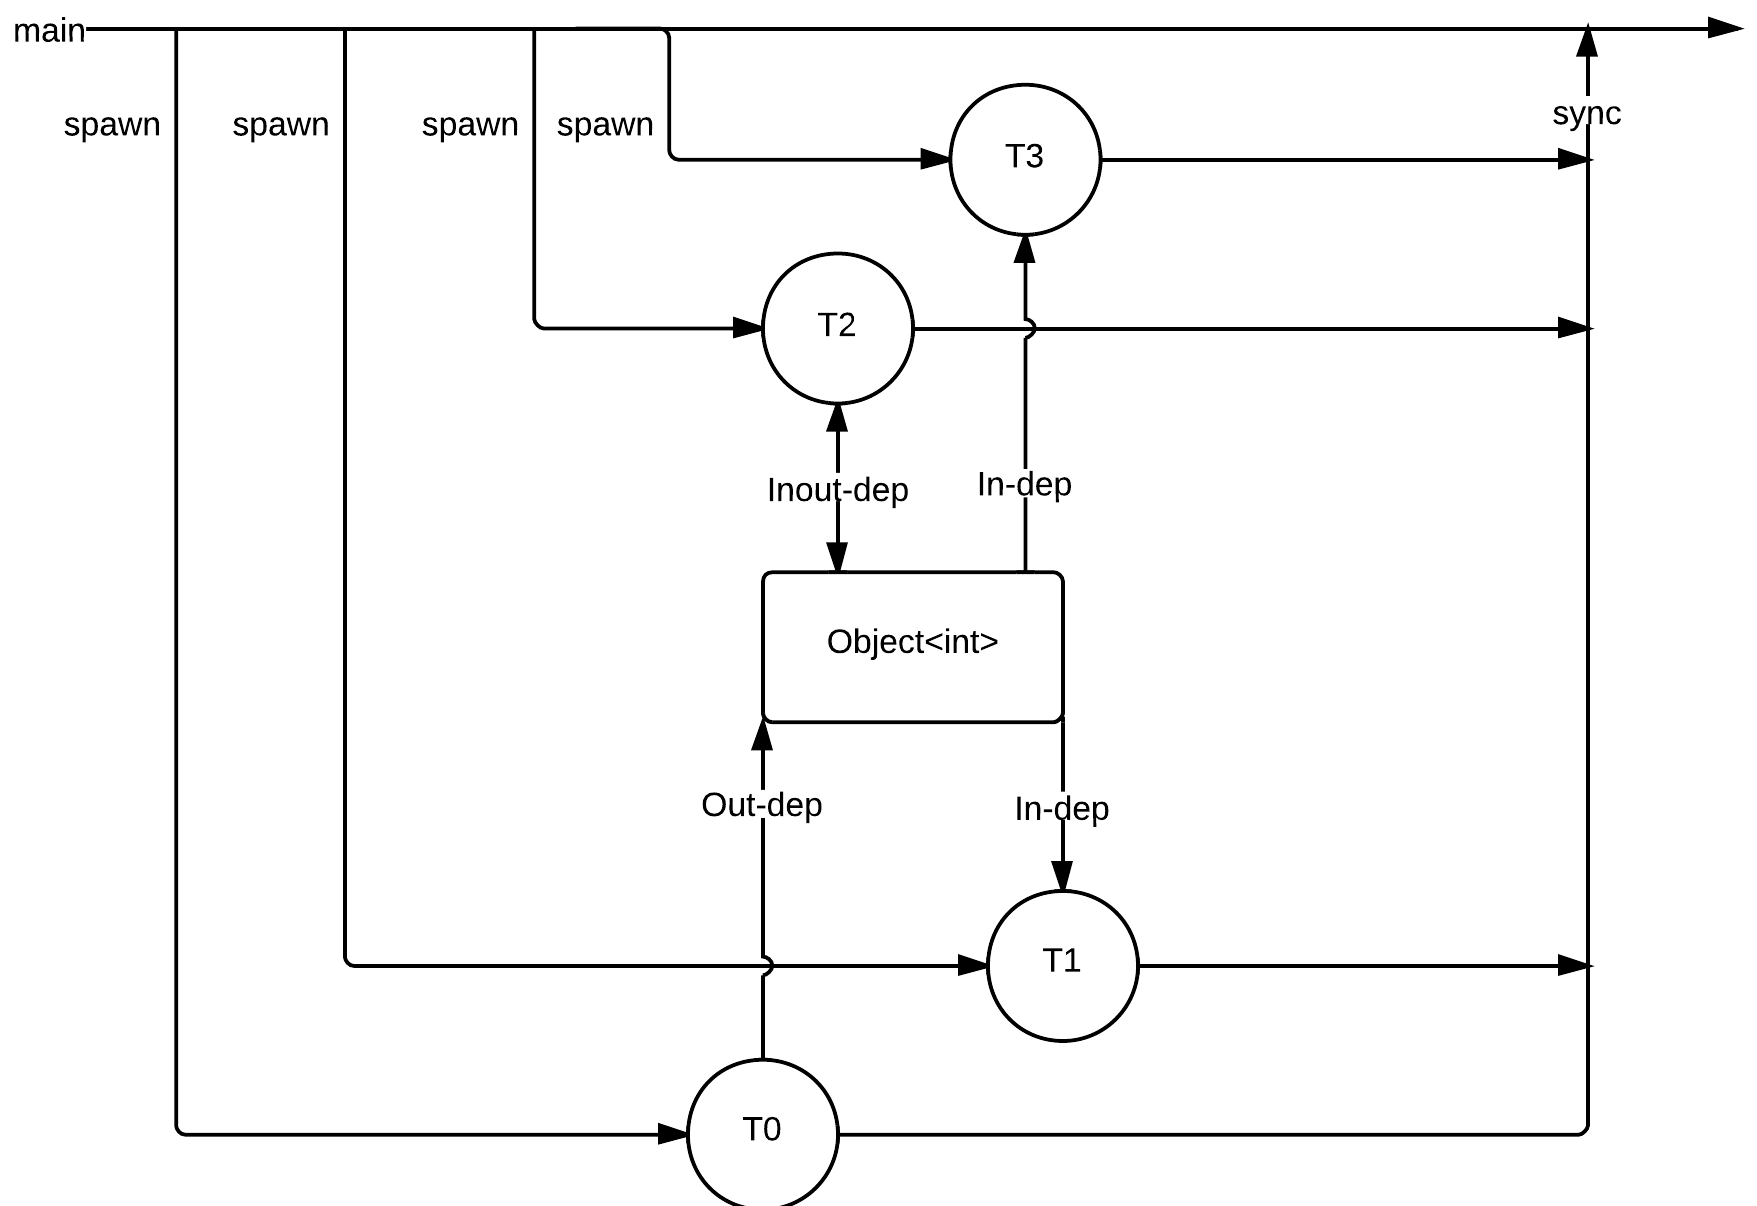
\includegraphics[width=300px]{img/deps}
	\caption{An illustration of object dependencies found in a task graph}
	\label{fig:deps}
\end{figure}

\begin{itemize}
\begin{item}
\emph{Out Dependencies}:  %ask Hans to review this part in particular!!
Outdeps specify relationships between tasks and objects in the case that a task will write to that object. An example of this can be seen in Figure \ref{fig:deps} where task \(T0\) has an out dependency to the object. As we discussed in the previous section an outdep will not affect a task's critical duration. We can see the reason for this by studying Figure \ref{fig:deps}.  Consider for instance the true statement that \(T2\) could be executed before or even in parallel with \(T1\). Initially we may be inclined to disagree with this statement as \(T2\)'s out dependency relationship with the object could mean that, in the event of \(T1\) reading from the object after \(T2\) has written to it, \(T1\) would read incorrect data. The reason we can be confident that this won't happen is that, in such a scenario, the scheduler will rename the objects, allowing parallelism. 

As shown in the algorithm the out dependency will affect the object's critical duration as any task with an in dependency to the same object, called after the out dependent task, will have to wait for the object to be ready. This can be illustrated in Figure \ref{fig:deps} by studying the interactions between task \(T0\) and task \(T1\). \(T1\) has an out dependency on the object which \(T0\) is writing to. This means that, in order to ensure correctness, \(T1\) cannot execute until \(T0\) has completed. To reflect this in the analysis tool we ensure that the object's critical duration is at least as long as \(T0\)'s thus ensuring that \(T1\)'s critical duration is at least as long as \(T0\)'s.
\end{item}
\begin{item}
\emph{In Dependencies}: 
An Indep relationship is one in-which the task depends on the output of an object. This can be seen in the case of task \(T3\). If we weren't taking object dependencies into account we could say that, because \(T3\) is spawned from the main method, its critical duration would be equal to the length of the main method up to that point. However this is not the case because of the in-dependency which means that if \(T3\) is to be correct it must have a critical path at least as long as the object i.e. the object's writer must have finished writing to it before the object can be read. In this case, because \(T2\) is the task responsible for writing to the object before it can be read by \(T3\), the critical duration of \(T2\), the object and \(T3\) will all be equal.
\end{item}

\begin{item}
\emph{In-Out Dependencies}: 
An in-out dependency encompasses both types of dependencies described above. It will affect both the task's critical duration and the object's critical duration. This is because its in-dependency requires access to the most up to date value of the object and its out-dependency forces the critical duration of the object to be at least as long as this task's critical duration.
\end{item}
\end{itemize}
It is now apparent that it is essential for a task not only to be aware of its own critical duration but also the critical duration of the entire program. If this were not the case, it would not be possible for the analysis tool to correctly set the object's critical duration. 

\subsubsection{Swan's Hooks}

Similarly to the functions which handled the non-object dependent portion of the critical duration analysis, the object dependent functions are also executed when arguments are issued and released. In order to handle object dependency swan uses functors, a C++ construct which can be thought of as ``executable objects" that we run on each argument in a parameter pack. For each parameter a template override will be matched in the functor executing the corresponding functionality. This is useful because, in the initialisation of each functor, the generic task-begin or task-end code, that is the code which is necessary for the critical duration analysis without objects, can be run. The object specialisations can then override any necessary values such as the critical duration. This is useful because it allows the program to have a single task beginning function and a single task ending function regardless of whether the task has object dependencies or not.
